\documentclass{article}

\usepackage{graphicx}
\usepackage{tikz}
\usepackage{tikzsymbols}
\usetikzlibrary{calc,patterns,shapes.geometric}
\pagestyle{empty}
\usepackage[margin=0pt]{geometry}
\geometry{papersize={14in,12in}}

\def\centerarc[#1](#2)(#3:#4:#5){\draw[#1] ($(#2)+({#5*cos(#3)},{#5*sin(#3)})$) arc (#3:#4:#5);}

\begin{document}
	\begin{figure}
		\centering
		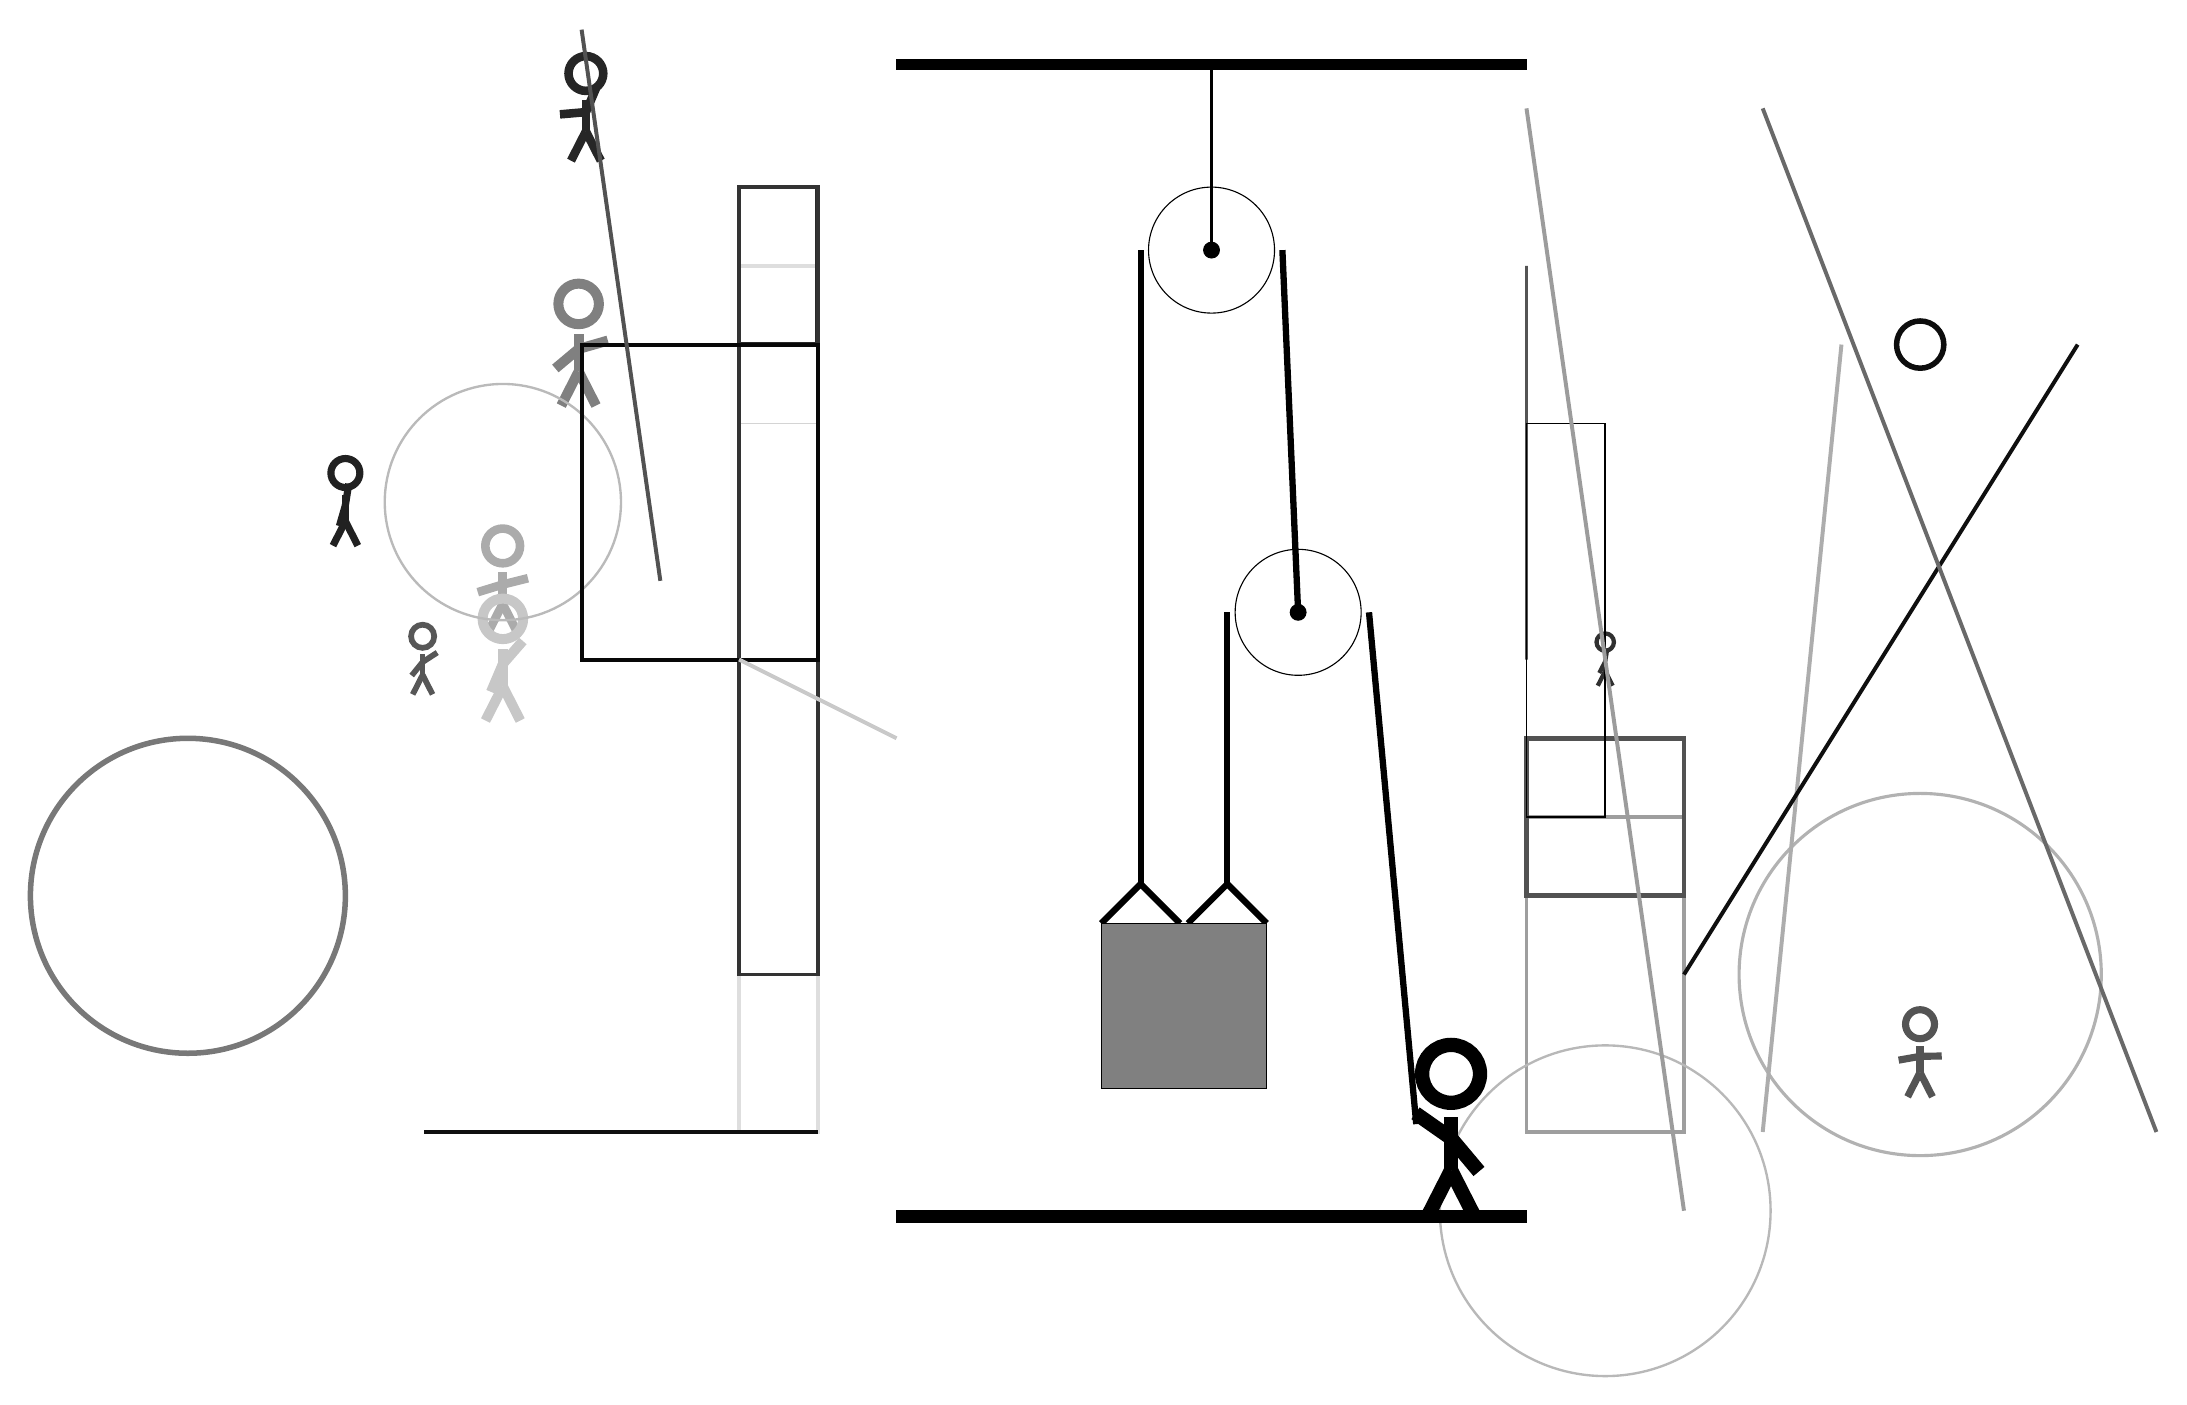
\begin{tikzpicture}
			%%%%% START %%%%%
			
			\draw[fill=black] (-2, 11.5) rectangle (6, 11.625);
			
			\draw (2, 9.2) circle (0.8);
			\draw[fill=black] (2, 9.2) circle (0.1);
			\draw[thick] (2, 9.2) -- (2, 11.5);
			
			\node[line width=0.3mm, color=black!81] at (7, 4) {\Strichmaxerl[3][63][81]};
			
			\draw[line width=0.2mm, color=black!17] (-4, 7) rectangle (-3, 10);
			\draw[line width=0.5mm, color=black!13] (-3, -2) rectangle (-4, 9);
			\node[line width=0.3mm, color=black!33] at (-7, 5) {\Strichmaxerl[6][17][14]};
			
			\draw[line width=0.5mm, color=black!94](-3, -2) -- (-8, -2);
			\draw[line width=0.4mm, color=black!38] (8, 2) rectangle (6, -2);
			\node[line width=0.3mm, color=black!22] at (-7, 4) {\Strichmaxerl[7][67][49]};
			\draw [line width=0.3mm, color=black!28](7, -3) circle (2.1);
			\draw[line width=0.6mm, color=black!68] (8, 1) rectangle (6, 3);
			\draw[line width=0.5mm, color=black!67] (6, 9) rectangle (6, 4);
			
			\draw [line width=0.4mm, color=black!30](11, 0) circle (2.3);
			\node[line width=0.2mm, color=black!66] at (-8, 4) {\Strichmaxerl[4][51][33]};
			\node[line width=0.6mm, color=black!85] at (-6, 11) {\Strichmaxerl[6][5][67]};
			
			\node[line width=0.7mm, color=black!50] at (-6, 8) {\Strichmaxerl[7][40][16]};
			\draw[line width=0.6mm, color=black!84] (-3, 10) rectangle (-4, 8);
			\node[line width=0.3mm, color=black!67] at (11, -1) {\Strichmaxerl[5][10][1]};
			
			\draw[line width=0.5mm, color=black!50](-4, 7) -- (-4, 4);
			\draw[line width=0.2mm, color=black!100] (6, 7) rectangle (7, 2);
			\draw[line width=0.5mm, color=black!80] (-4, 10) rectangle (-3, 0);
			\draw [line width=0.3mm, color=black!27](-7, 6) circle (1.5);
			\draw[line width=0.5mm, color=black!32](9, -2) -- (10, 8);
			
			\draw[line width=0.5mm, color=black!97] (-3, 4) rectangle (-6, 8);
			\draw[line width=0.5mm, color=black!21](-2, 3) -- (-4, 4);
			\draw[line width=0.5mm, color=black!94](8, 0) -- (13, 8);
			\draw[line width=0.5mm, color=black!59](9, 11) -- (14, -2);
			\draw [line width=0.7mm, color=black!53](-11, 1) circle (2.0);
			
			\draw[line width=0.5mm, color=black!68](-6, 12) -- (-5, 5);
			\draw [line width=0.7mm, color=black!95](11, 8) circle (0.3);
			\draw[line width=0.5mm, color=black!39](8, -3) -- (6, 11);
			
			\node[line width=0.2mm, color=black!87] at (-9, 6) {\Strichmaxerl[5][74][81]};
			
			\draw (3.1, 4.6) circle (0.8);
			\draw[fill=black] (3.1, 4.6) circle (0.1);
			
			\draw[line width = 0.8mm]  (0.6, 0.65) -- (1.1, 1.15) -- (1.6, 0.65);
			\draw[line width = 0.8mm]  (1.7, 0.65) -- (2.2, 1.15) -- (2.7, 0.65);
			\draw[fill=black!50] (0.6, 0.65) rectangle (2.7, -1.45);
			
			\draw[line width = 0.8mm] (1.1, 9.2) -- (1.1, 1.15);
			\centerarc[line width = 0.8mm](2, 9.2)(0:180:0.9);
			\draw[line width = 0.8mm] (2.9, 9.2) -- (3.1, 4.6);
			\draw[line width = 0.8mm] (2.2, 4.6) -- (2.2, 1.15);
			\centerarc[line width = 0.8mm](3.1, 4.6)(0:180:0.9);
			\draw[line width = 0.8mm] (4.0, 4.6) -- (4.6, -1.9);
			
			\node at (5, -2) {\Strichmaxerl[10][-35][-50]};
			
			\draw[fill=black] (-2, -3) rectangle (6, -3.15);
			
			%%%%% END %%%%%
		\end{tikzpicture}
	\end{figure}	
\end{document}